\documentclass[10pt, conference]{IEEEtran}

\usepackage[pdftex]{graphicx}
\usepackage[cmex10]{amsmath}
\usepackage{amsfonts}

\usepackage{color}
% \usepackage{hyperref}
% \hypersetup{colorlinks=true,
%     linkcolor=blue,
%     citecolor=blue,
%     filecolor=blue,
%     urlcolor=blue,
%     unicode=false}
% \urlstyle{same}

\usepackage{tabularx}
\usepackage{booktabs}
\usepackage{siunitx}
\usepackage{subfig}
\usepackage{paralist}
\usepackage{colortbl}
\usepackage{listings}

\usepackage{enumitem}

\newif\ifcomments\commentstrue

\ifcomments
\newcommand{\authornotation}[3]{\textcolor{#1}{[#3 ---#2]}}
\newcommand{\todo}[1]{\textcolor{red}{[TODO: #1]}}
\else
\newcommand{\authornotation}[3]{}
\newcommand{\todo}[1]{}
\fi

\newcommand{\wss}[1]{\authornotation{blue}{SS}{#1}}
\newcommand{\ms}[1]{\authornote{cyan}{MS}{#1}}

\newcommand{\progname}{SFS}
\newcommand{\colAwidth}{0.13\textwidth}
\newcommand{\colBwidth}{0.84\textwidth}

\begin{document}

\title{A Software Engineering Capstone Infrastructure that Encourages Spreading
Work Over Time and Team}

\author{\IEEEauthorblockN{}
\IEEEauthorblockA{}

% \author{\IEEEauthorblockN{Spencer Smith, Christopher Schankula, Lucas Dutton and Christopher Anand}
% \IEEEauthorblockA{Computing and Software Department\\
% McMaster University, Canada\\
% Email: smiths@mcmaster.ca, schankuc@mcmaster.ca, duttonl@mcmaster.ca, anandc@mcmaster.ca}

% \and
% \IEEEauthorblockN{Sumanth Shankar}
% \IEEEauthorblockA{Mechanical Engineering Department\\
% McMaster University, Canada\\
% Email: shankar@mcmaster.ca }
}

\maketitle
  
\begin{abstract}

How can instructors facilitate spreading out the work in a software engineering
or computer science capstone course across time and between team members?
Currently teams often compromise the quality of their learning experience by
frantically working before each deliverable.  Some team members further
compromise learning by not contributing their fair share to the team effort. To
mitigate these problems, we propose using a GitHub template that contains all
the initial infrastructure a team needs, including the folder structure,
text-based template documents and template issues. In addition, we propose each
team begins the year by identifying specific quantifiable individual
productivity metrics for monitoring, such as the count of meetings attended,
issues closed and number of commits.  Initial data suggests that these steps
have an impact.  In 2022/23 we observed 50\% of commits happening within 3 days
of due dates.  After partially introducing the above ideas in 2023/24, this
number improved to 37\%. We experiment with different measures of fairness of
workload distribution, including the ratio of maximum to minimum commits on a
team, Jain's fairness index, and our own fairness index based on disparity
between number of commits. Going forward we propose an experiment where commit
data and interview data is compared between teams that use the proposed
interventions and those that do not.

\end{abstract}

\begin{IEEEkeywords}
software engineering; capstone; template repository
\end{IEEEkeywords}

\section{Introduction} \label{SecIntro}

The workload for a software engineering or computer science capstone team
project is often unevenly distributed over time and between team members.  Teams
typically work in frantic bursts of activity right before a deadline and then
cease almost all activity until their next deadline.  These work habits
compromise the learning objectives of the course because the students do not
have time to properly plan their activities or reflect on their work.  The
uneven distribution of effort between team mates is also problematic.  Some
students take on an unfair share of the work, causing them stress and possibly
hurting their experience in other courses, while those investing less effort
miss important learning opportunities.  How can instructors mitigate these
problems?

To address the uneven distribution of work, need to first think about why the
problems exist.  Not the same as the workplace.  Other pressures on students.
Not sure of expectations.  Not sure where to begin.  Peer pressure and social
interactions that make it challenging to take charge of the group, or criticize
other group members.  [There must be some literature that talks about the
challenges for student teamwork, teamwork in SE, teamwork for capstone projects,
teamwork for SE capstone projects]

Ideas on what we can do about it at an abstract level - the forces we can use to
direct students.  We have grades and we have structure of the course and
expectations.

Overview of ideas.

Roadmap of paper.

Making sure that BibTex is working \cite{Smith2005}.

\section{Literature Review} \label{SecLitReview}
May not need this if the literature is covered in the introduction.

\section{Proposed Infrastructure} \label{SecInfrastruct}

roadmap blurb

\subsection{Structure and Timeline}

Context of course. Double blind. figure showing the V model and the expected
deliverables.  The ideas in this paper could work for other structures, but this
is the one adopted.

\begin{figure}[h!]
  \begin{center}
    {
      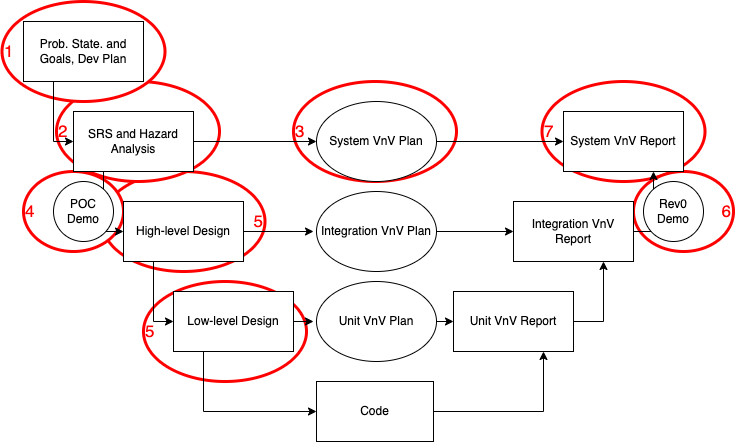
\includegraphics[width=0.75\columnwidth]{./figures/VModelOfProcessDeliverables.png}
    }
    \caption{\label{Fig_VModel} V Model Used for Capstone Deliverables}
  \end{center}
\end{figure}
% TODO - redraw the figure if time, and save as pdf
\subsection{Template Repository}

link

\begin{figure}[h!]
  \begin{center}
    {
      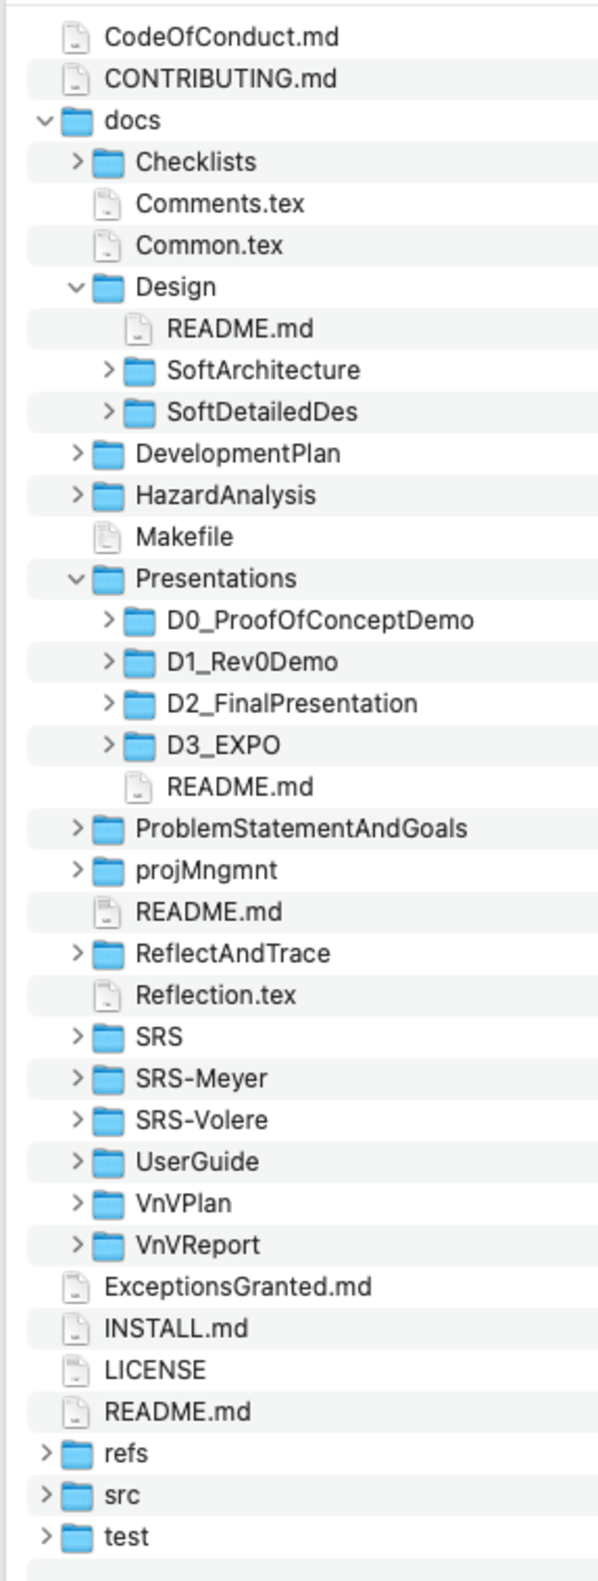
\includegraphics[width=0.7\columnwidth]{./figures/GitHubTemplate}
    }
    \caption{\label{Fig_GitHubTemplate} GitHub Template}
  \end{center}
\end{figure}

\subsection{Team Contribution Measurement}


\section{Preliminary Data} \label{SecPrelimData}

Look at commits over time, and possibly lines (removing outliers) of code over
time

\begin{figure}[h!]
\begin{center}
{
     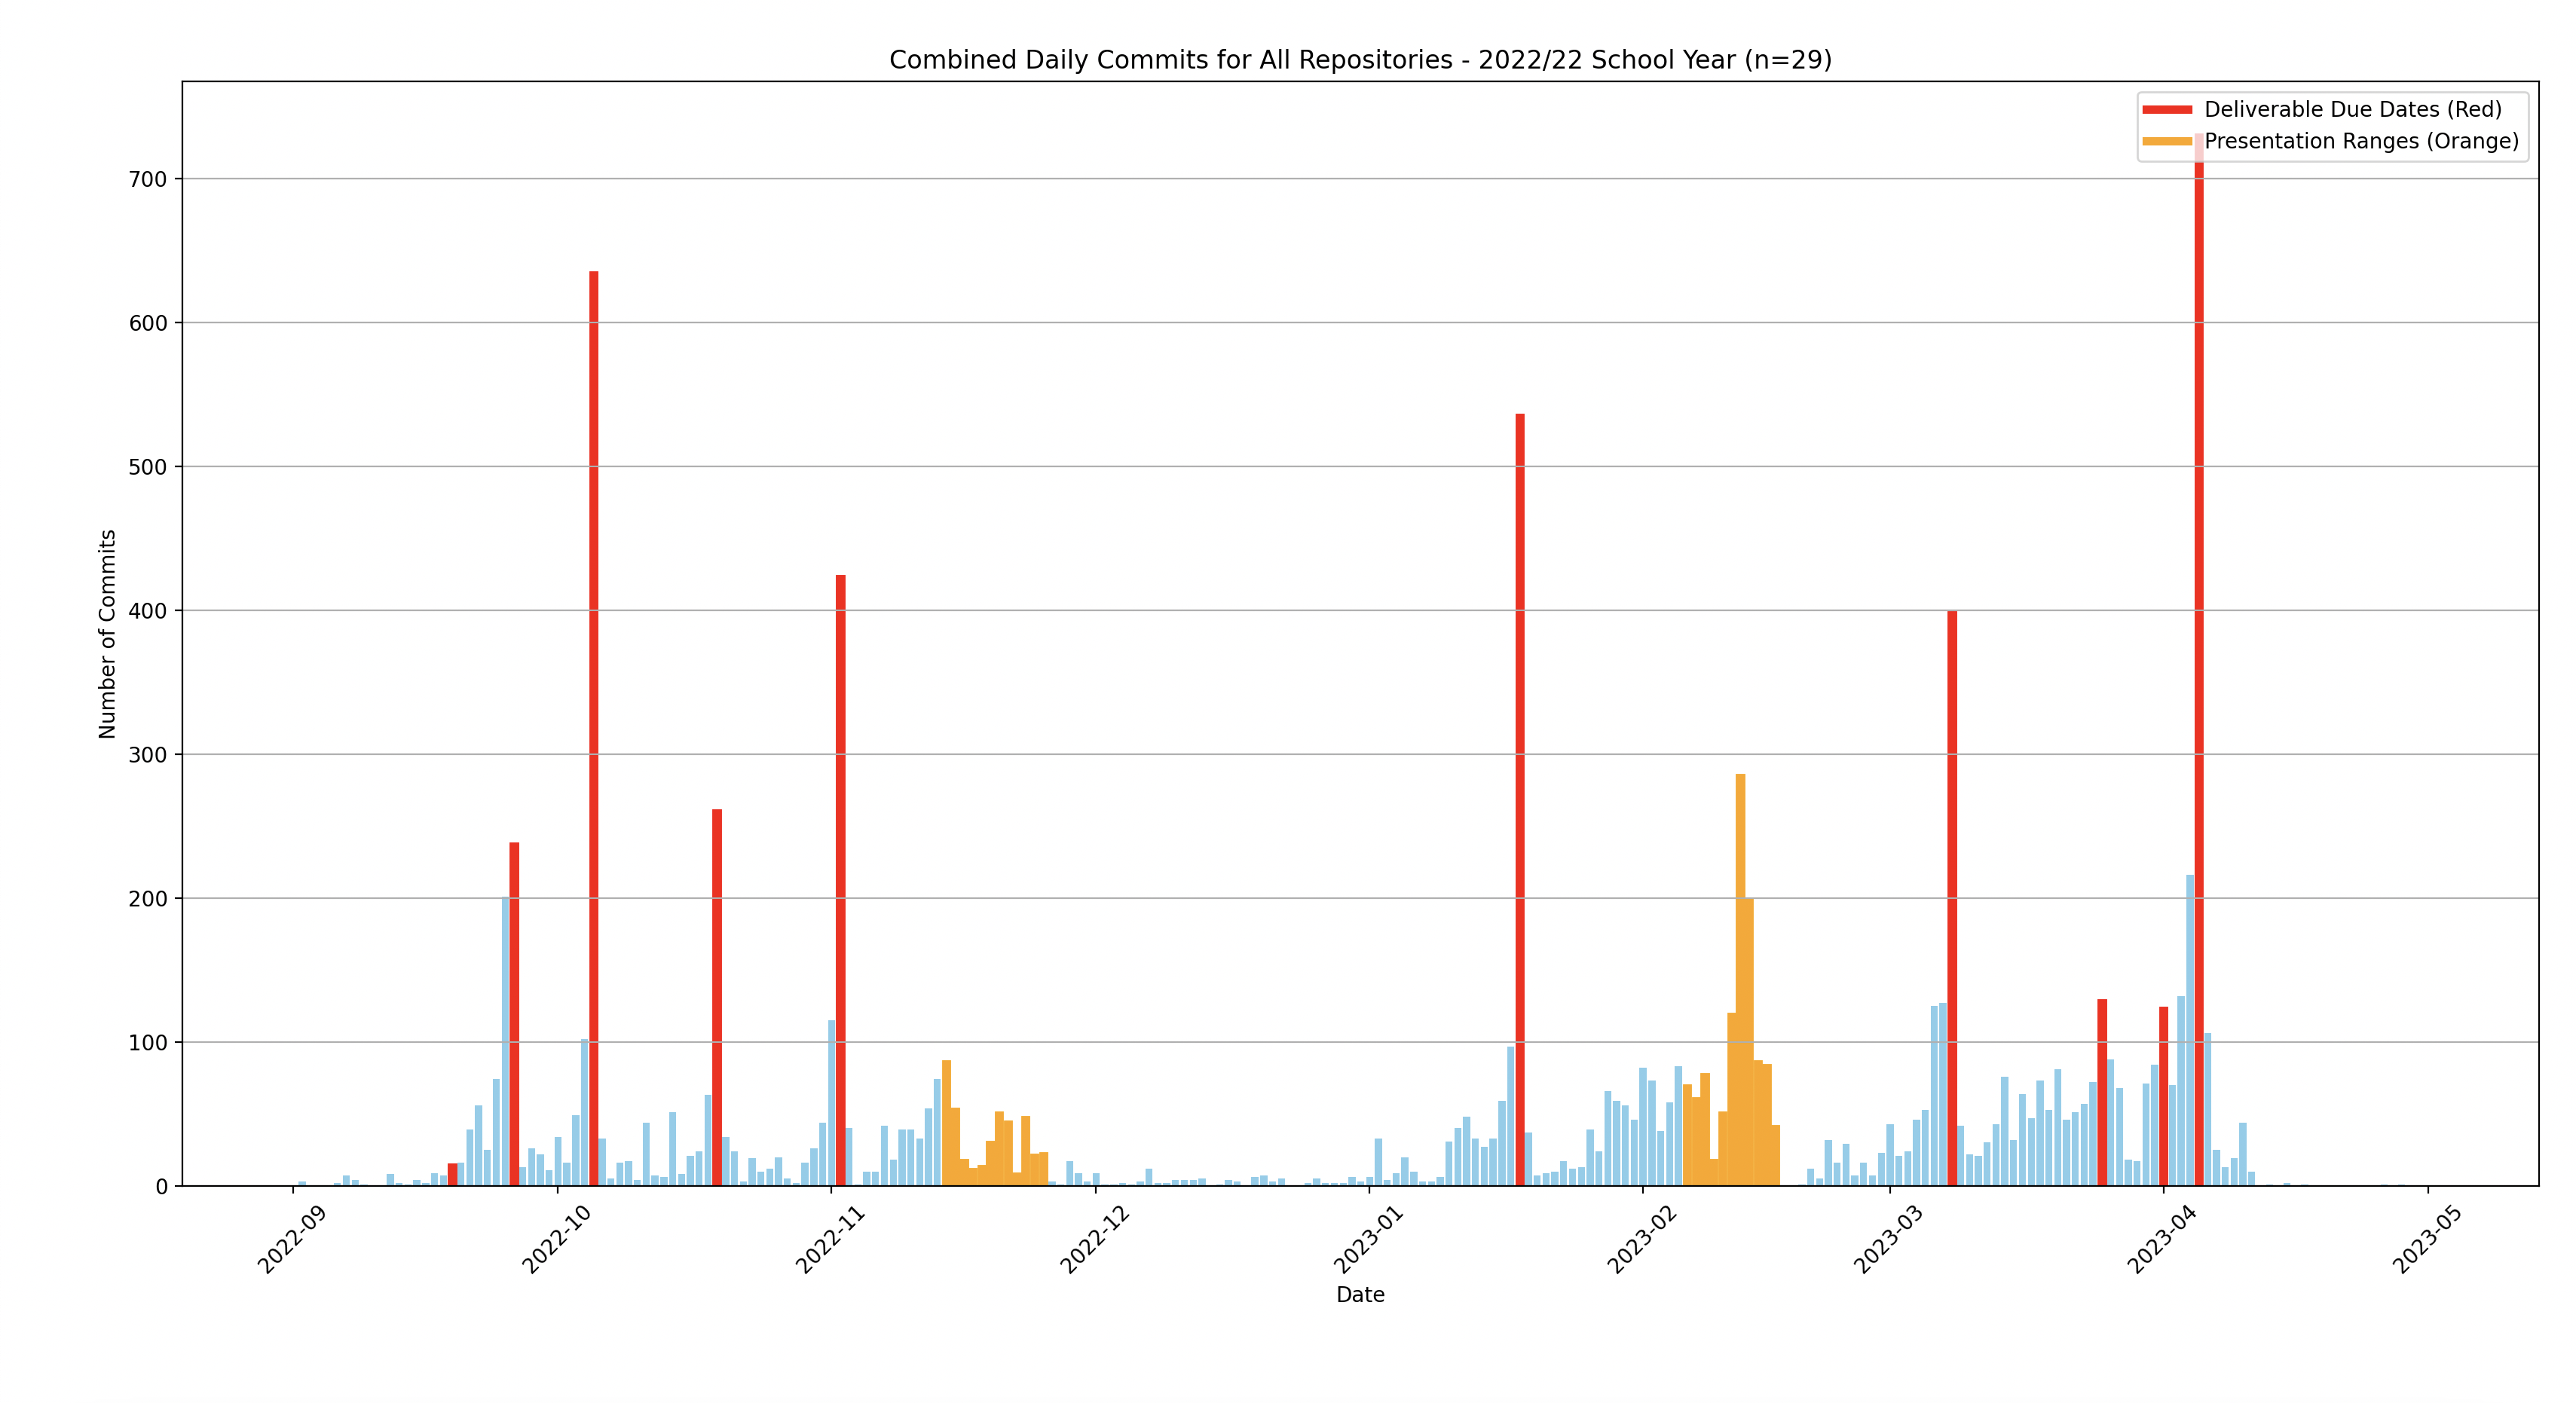
\includegraphics[width=0.75\columnwidth]{./figures/Yr22_23_DailyCommitsTimeline.png}
}
\caption{\label{Fig_22_23Timeline} Timeline of Commits for 2022--2023}
\end{center}
\end{figure}
  
\begin{figure}[h!]
\begin{center}
{
     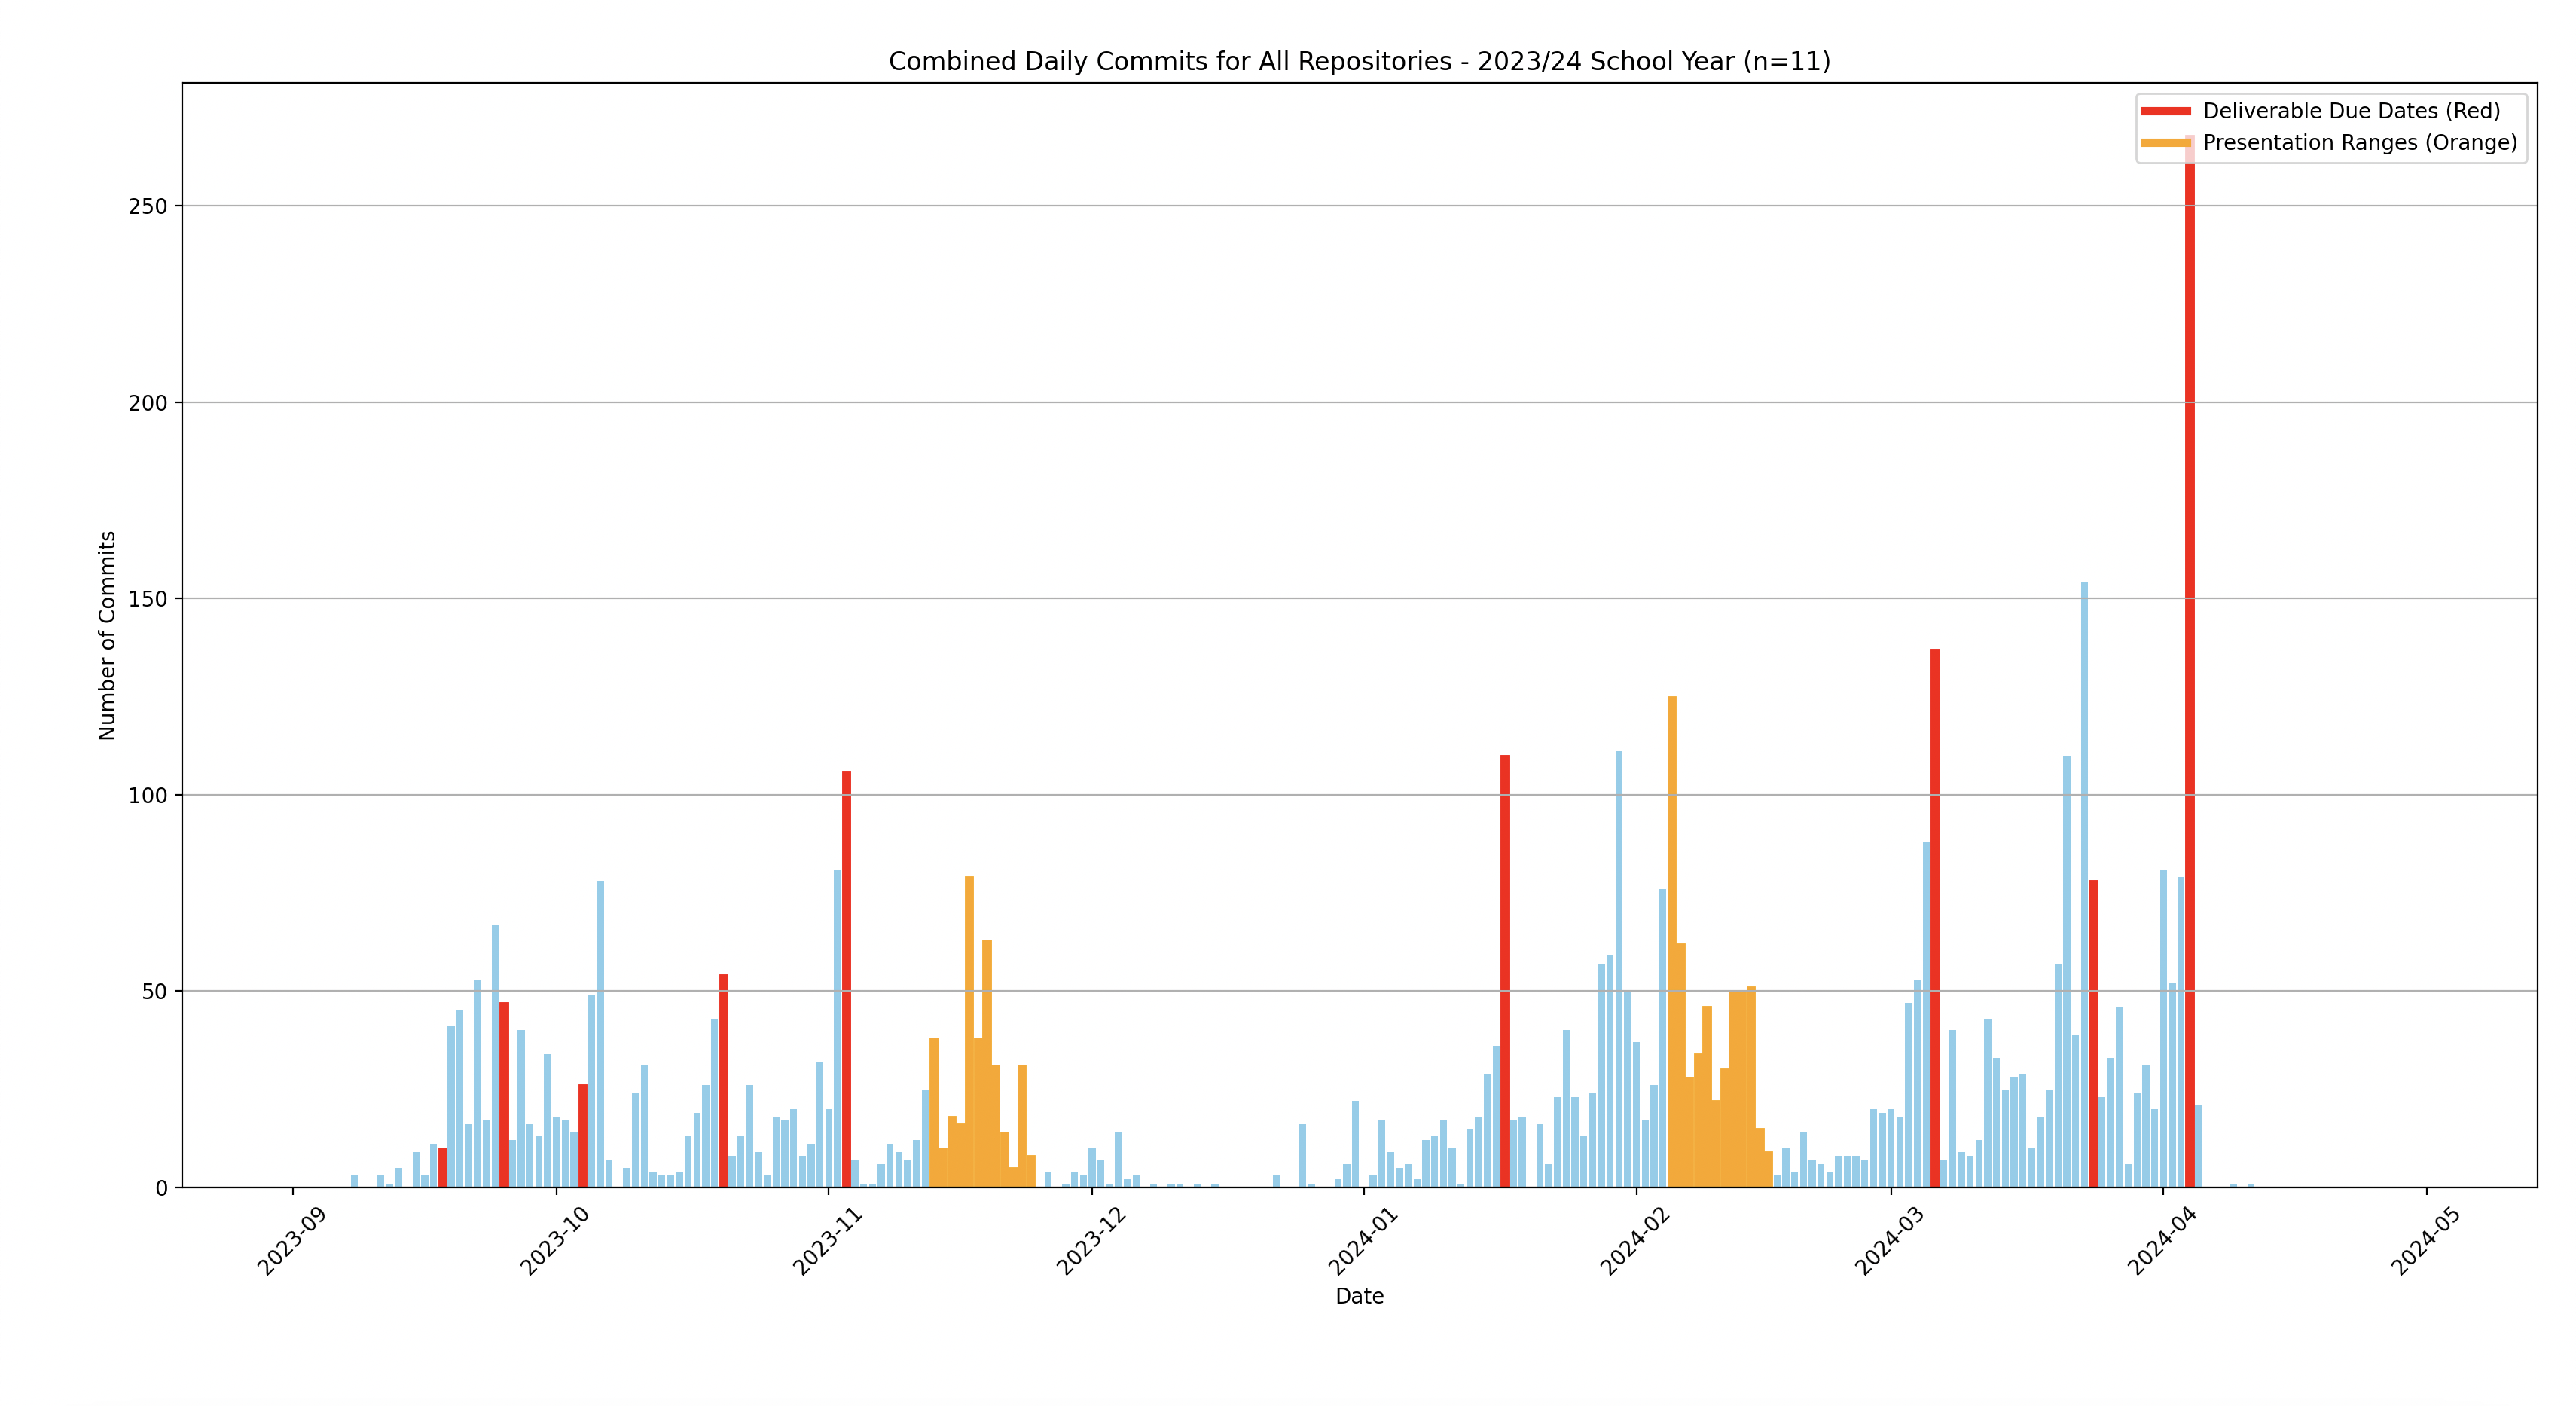
\includegraphics[width=0.75\columnwidth]{./figures/Yr23_24_DailyCommitsTimeline.png}
}
\caption{\label{Fig_23_24Timeline} Timeline of Commits for 2023--2024}
\end{center}
\end{figure}

\subsection{Timeline Comparison}

Timeline comparison

\subsection{Measuring Fairness}

New fairness metric.

$$
{ \sum\limits_{c, x \in C} (c > x \Rightarrow  {c-x})} / {((\left|C\right| -
1) \cdot \sum\limits_{c \in C} c)}
$$

\section{Proposed Experiment} \label{SecProposedExperiment}

Start with research questions.

Collect the same data as in Section~\ref{SecPrelimData} and conduct focus groups
in all three CAS capstone courses (SE, CS and TRON).  

Threats to validity:

\begin{itemize}
    \item Multiple changes are made to the course, so it is difficult to
    determine which change influences the student behaviour.  The focus group
    should hopefully tease that out.
    \item Comparing different courses with different instructors, different
    backgrounds for students, etc.
    \item etc.
\end{itemize}

\section{Concluding Remarks} \label{SecConclusions}

\section*{Acknowledgements}

If any.

\bibliographystyle{IEEEtran}
\bibliography{SmithEtAl2024_CSEEnT}

\end{document}
